\documentclass[../main.tex]{subfiles}

\begin{document}
  \section{Protocolli di Autenticazione e Scambio Chiavi}

\subsection{Protocolli di Autenticazione}
\label{sec:autenticazione}

\subsubsection{Autenticazione di Sistema vs. di Messaggi}
È importante distinguere due concetti diversi di autenticazione:
\begin{itemize}
    \item \textbf{Autenticazione di Messaggi:} Si occupa di verificare l'origine e l'integrità di un singolo messaggio. Gli strumenti usati sono i \textbf{MAC} (autenticazione + integrità) e le \textbf{firme digitali} (autenticazione + integrità + non ripudio). La verifica non deve necessariamente avvenire in tempo reale.
    \item \textbf{Autenticazione di Sistema (Entity Authentication):} È il processo di identificazione di un'entità (utente, sistema) che partecipa a un protocollo di rete, supportato da prove. Questa verifica deve avvenire \textbf{in real-time}.
\end{itemize}

I protocolli di autenticazione di sistema devono soddisfare diversi requisiti:
\begin{itemize}
    \item \textbf{Autenticazione:} A deve poter verificare l'identità di B. Idealmente, si ha una \textbf{mutua autenticazione} (anche B autentica A).
    \item \textbf{Non trasferibilità:} A non deve poter riutilizzare i dati scambiati per impersonare B verso una terza entità C.
    \item \textbf{Robustezza:} Un'entità C non deve poter impersonare B, anche se C può osservare molti scambi tra A e B (resistenza al \emph{replay attack}).
\end{itemize}

\subsubsection{Basi per l'Autenticazione}
Per autenticare B ad A, B deve fornire una prova basata su uno o più dei seguenti fattori:
\begin{enumerate}
    \item \textbf;Qualcosa che B conosce:} PIN, password, chiave simmetrica, chiave privata.
    \item \textbf{Qualcosa che B possiede:} Smart-card, token (es. "calcolatrice" one-time-password).
    \item \textbf{Qualcosa che B è:} Una caratteristica fisica (biometria).
\end{enumerate}

\subsubsection{Protocolli Challenge-Response (Autenticazione Forte)}
L'autenticazione \textbf{forte} (challenge-response) si basa sulla conoscenza di un dato segreto $s$ (es. una chiave crittografica, non una password).
Il meccanismo base prevede che B (verifier) invii ad A (claimant) una \textbf{challenge} (sfida). A deve calcolare una \textbf{response} (risposta) applicando una funzione segreta $f_s$ alla challenge. B verifica la risposta.
Per prevenire attacchi di tipo \emph{replay}, la challenge deve essere \textbf{tempo-variante}, utilizzando:
\begin{itemize}
    \item \textbf{Nonce:} Un numero usato una sola volta (es. $c_1, c_2$).
    \item \textbf{Timestamp (t):} Un marcatore temporale (richiede orologi sincronizzati).
    \item \textbf{Sequence Number:} Un contatore (richiede gestione dello stato).
\end{itemize}

\begin{figure}[H]
  \centering
  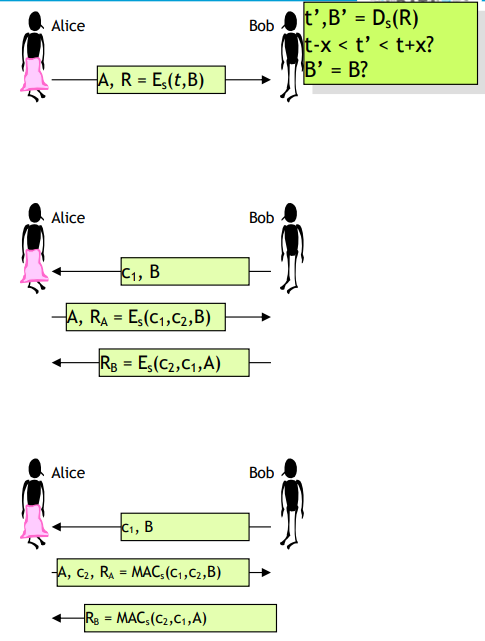
\includegraphics[width=0.8\textwidth]{CRsymm.png}
  \caption{Schema protocollo C/R simmetrico (Pag 18)}
  \label{fig:CRsymm}
\end{figure}

\subsubsection*{Descrizione Immagine: Schema protocollo C/R simmetrico (Pag 18)}
Questa immagine (Pag 18) mostra tre protocolli di autenticazione challenge-response tra "Alice" e "Bob" che condividono una chiave simmetrica segreta $s$.
\begin{itemize}
    \item \textbf{Schema 1 (Timestamp, One-Way):}
          \begin{enumerate}
              \item Alice invia a Bob: $A, R = E_s(t, B)$.
              \item $E_s$ è la cifratura con la chiave segreta $s$. $t$ è un timestamp, $B$ è l'identificativo di Bob (incluso per prevenire che Bob riutilizzi $R$ per impersonare Alice verso qualcun altro).
              \item Bob riceve $R$, lo decifra con $s$ ottenendo $t'$ e $B'$. Controlla che $B' = B$ e che il timestamp $t'$ sia "recente" (es. $t-x < t' < t+x$). Se i controlli passano, Alice è autenticata.
          \end{enumerate}
    \item \textbf{Schema 2 (Random Challenge, Mutua Autenticazione - Cifratura):}
          \begin{enumerate}
              \item Bob invia ad Alice una challenge (nonce): $c_1, B$.
              \item Alice invia a Bob: $A, R_A = E_s(c_1, c_2, B)$. $c_2$ è la challenge di Alice per Bob.
              \item Bob decifra $R_A$ con $s$, controlla che $c_1$ sia il nonce che ha inviato. Ora Bob ha autenticato Alice.
              \item Bob invia ad Alice: $R_B = E_s(c_2, c_1, A)$. (Notare l'ordine invertito $c_2, c_1$).
              \item Alice decifra $R_B$ con $s$, controlla che $c_2$ sia il nonce che ha inviato. Ora Alice ha autenticato Bob.
          \end{enumerate}
    \item \textbf{Schema 3 (Random Challenge, Mutua Autenticazione - MAC):}
          \begin{itemize}
              \item Identico allo Schema 2, ma invece di usare la cifratura $E_s$, usa un Message Authentication Code (MAC) calcolato con la chiave $s$.
              \item $R_A = MAC_s(c_1, c_2, B)$
              \item $R_B = MAC_s(c_2, c_1, A)$
              \item Questo è più efficiente perché non richiede cifratura, ma solo il calcolo di un hash con chiave.
          \end{itemize}
\end{itemize}


\begin{figure}[H]
  \centering
  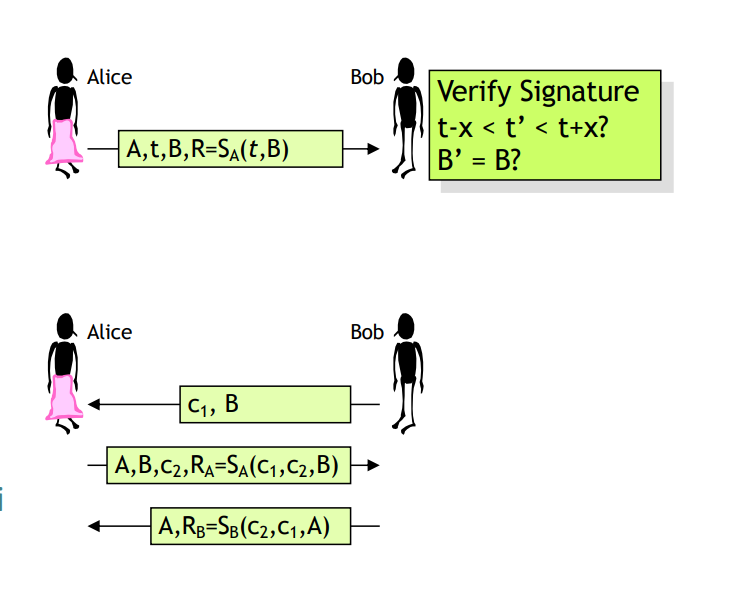
\includegraphics[width=0.8\textwidth]{CRasymm.png}
  \caption{Schema protocollo C/R asimmetrico (Pag 19)}
  \label{fig:CRasymm}
\end{figure}

\subsubsection*{Descrizione Immagine: Schema protocollo C/R asimmetrico (Pag 19)}
Questa immagine (Pag 19) mostra due protocolli analoghi ai precedenti, ma basati su crittografia asimmetrica (firme digitali) invece che su una chiave condivisa.
\begin{itemize}
    \item \textbf{Schema 1 (Timestamp, One-Way):}
          \begin{enumerate}
              \item Alice invia a Bob: $A, t, B, R = S_A(t, B)$.
              \item $S_A$ è la \textbf{firma digitale} di Alice, creata usando la sua \textbf{chiave privata} sul timestamp $t$ e sull'ID di Bob $B$.
              \item Bob riceve il messaggio, usa la \textbf{chiave pubblica} di Alice (che deve già possedere) per verificare la firma $R$.
              \item Se la firma è valida, Bob controlla la freschezza di $t$ e che $B$ sia il suo ID. Se sì, Alice è autenticata.
          \end{enumerate}
    \item \textbf{Schema 2 (Random Challenge, Mutua Autenticazione):}
          \begin{enumerate}
              \item Bob invia ad Alice una challenge (nonce): $c_1, B$.
              \item Alice invia a Bob: $A, B, c_2, R_A = S_A(c_1, c_2, B)$. $R_A$ è la sua firma (privata) sulle due challenge e sull'ID di Bob.
              \item Bob verifica $R_A$ (con $K_{pubA}$), controlla $c_1$ (autenticando Alice).
              \item Bob invia ad Alice: $A, R_B = S_B(c_2, c_1, A)$. $R_B$ è la sua firma (privata) sulle challenge (ordine invertito) e sull'ID di Alice.
              \item Alice verifica $R_B$ (con $K_{pubB}$), controlla $c_2$ (autenticando Bob).
          \end{enumerate}
\end{itemize}

\subsection{Instaurazione di Chiavi Effimere (di Sessione)}

\subsubsection{Perché usare Chiavi Effimere?}
\begin{itemize}
    \item Si limita la quantità di dati cifrati con la stessa chiave (utile contro attacchi \emph{ciphertext-only}).
    \item \textbf{Limitazione dei danni:} Se una chiave effimera $K_t$ viene compromessa, solo la sessione cifrata con essa è compromessa. La master key (a lungo termine) rimane sicura.
    \item Permette di gestire chiavi diverse per sessioni diverse.
\end{itemize}
L'architettura di riferimento prevede che ogni entità possegga una \emph{master key} (a lungo termine) usata per generare o trasportare le chiavi effimere $K_t$.

\subsubsection{Perfect Forward Secrecy (PFS)}
La \textbf;Perfect Forward Secrecy (PFS)} è una proprietà ideale di un protocollo di scambio chiavi.
\textbf;Definizione:} La compromissione della \emph{master key} (a lungo termine) in un istante $t$ \textbf{non} deve compromettere la segretezza delle chiavi effimere generate in passato (fino a $t-1$).
Se un attaccante (Trudy) registra una sessione $S_1$ (cifrata con $K_{t1}$) e \emph{successivamente} ruba la $K_{master}$, la PFS garantisce che Trudy non possa comunque usare $K_{master}$ per risalire a $K_{t1}$ e decifrare $S_1$.

\subsubsection{Classi di Protocolli di Scambio Chiavi}
\begin{description}
    \item[$K_t$ Trasportata]
    Una entità (es. Alice) genera $K_t$ e la invia all'altra (Bob), crittografandola con la master key.
    \begin{itemize}
        \item \textbf{Vantaggi:} Semplice ed efficiente.
        \item \textbf{Svantaggi:} \textbf{Non offre PFS}. Se Trudy ruba la master key, può decifrare il trasporto di $K_t$ e recuperare tutte le chiavi di sessione passate.
    \end{itemize}
    \begin{figure}[H]
      \centering
      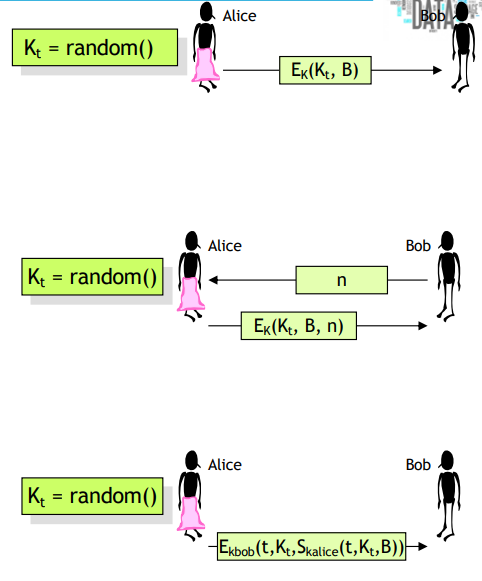
\includegraphics[width=0.8\textwidth]{Ktt.png}
      \caption{Schema protocollo trasporto $K_t$ (Pag 22)}
      \label{fig:Ktt}
    \end{figure}

    \subsubsection*{Descrizione Immagine: Schema protocollo trasporto $K_t$ (Pag 22)}
    \begin{itemize}
        \item \textbf{Contesto:} L'immagine (Pag 22) mostra tre modi in cui Alice può generare una chiave $K_t$ e "trasportarla" (inviarla) a Bob.
        \item \textbf{Schema 1 (Simmetrico Semplice):}
              \begin{itemize}
                  \item Alice genera $K_t = random()$.
                  \item Alice invia a Bob: $E_K(K_t, B)$.
                  \item $E_K$ è la cifratura con una \emph{master key simmetrica} $K$ condivisa tra Alice e Bob.
                  \item \textbf{Criticità:} Non offre PFS ed è vulnerabile a replay attack (Trudy può re-inviare questo messaggio a Bob).
              \end{itemize}
        \item \textbf{Schema 2 (Simmetrico con Nonce):}
              \begin{itemize}
                  \item Bob invia un nonce (numero casuale) $n$ ad Alice.
                  \item Alice genera $K_t = random()$.
                  \item Alice invia a Bob: $E_K(K_t, B, n)$.
                  \item Bob decifra e controlla che $n$ sia quello che ha inviato, sconfiggendo il replay attack.
                  \item \textbf{Criticità:} Non offre ancora PFS.
              \end{itemize}
        \item \textbf{Schema 3 (Asimmetrico/Ibrido):}
              \begin{itemize}
                  \item Alice genera $K_t = random()$.
                  \item Alice invia a Bob: $E_{kbob}(t, K_t, S_{kalice}(t, K_t, B))$.
                  \item Questo messaggio è composto:
                        \begin{itemize}
                            \item $E_{kbob}(...)$: L'intero messaggio è cifrato con la \emph{chiave pubblica di Bob}. Solo Bob può leggerlo.
                            \item $t$: Un timestamp per prevenire replay attack.
                            \item $K_t$: La chiave effimera.
                            \item $S_{kalice}(...)$: Una \emph{firma digitale} (fatta con la \emph{chiave privata di Alice}) su $t$, $K_t$ e $B$, per autenticare Alice come mittente.
                        \end{itemize}
                  \item \textbf{Criticità:} Non offre PFS. Se la \emph{chiave privata di Bob} ($k_{priv\_bob}$) venisse rubata in futuro, Trudy potrebbe decifrare tutte le sessioni passate registrate, poiché $K_t$ è trasportata (cifrata).
              \end{itemize}
    \end{itemize}

    \item[$K_t$ Derivata]
    Le entità si scambiano dati (es. numeri casuali) e \emph{derivano} $K_t$ crittograficamente, usando la master key nel processo.
    \begin{itemize}
        \item \textbf{Vantaggi:} \textbf{Può offrire PFS} (es. protocollo EKE, che è un DH autenticato).
        \item \textbf{Svantaggi:} Più complesso e meno efficiente in termini di messaggi scambiati.
    \end{itemize}
    \begin{figure}[H]
      \centering
      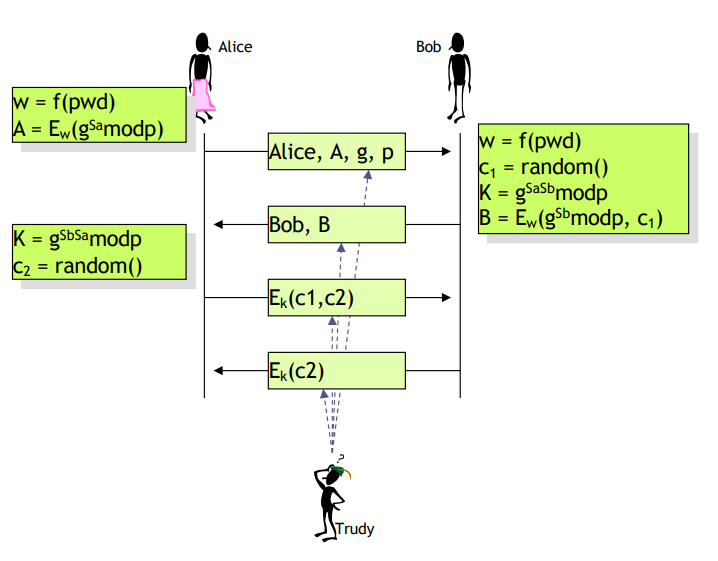
\includegraphics[width=0.8\textwidth]{EKE.png}
      \caption{Autenticazione forte con password Encrypted Key Exchange (Pag 17)}
      \label{fig:EKE}
    \end{figure}
    
    \subsubsection*{Descrizione Immagine: Encrypted Key Exchange (EKE) (Pag 17)}
    \begin{itemize}
        \item \textbf{Contesto:} L'immagine (Pag 17) mostra il protocollo EKE, che \emph{deriva} una chiave di sessione $K$ usando Diffie-Hellman (DH) e la autentica usando una password ($pwd$) condivisa. \textbf{Questo protocollo offre PFS}.
        \item \textbf{Flusso del Protocollo:}
              \begin{enumerate}
                  \item Alice e Bob calcolano entrambi indipendentemente una chiave temporanea $w = f(pwd)$ (es. hash della password).
                  \item Alice sceglie un segreto DH $sa$. Calcola la sua parte pubblica DH ($g^{sa} \mod p$) e la \emph{cifra} con $w$.
                  \item Alice $\to$ Bob: $Alice, A = E_w(g^{sa} \mod p)$.
                  \item Bob (che conosce $w$) decifra $A$ per ottenere $g^{sa}$. Sceglie il suo segreto DH $sb$. Calcola la sua parte pubblica $g^{sb} \mod p$.
                  \item Bob calcola la chiave di sessione finale $K = (g^{sa})^{sb} \mod p$.
                  \item Bob $\to$ Alice: $Bob, B = E_w(g^{sb} \mod p, c_1)$ (invia la sua parte pubblica cifrata, insieme a una challenge $c_1$).
                  \item Alice decifra $B$, ottiene $g^{sb}$ e $c_1$. Calcola anche lei la chiave finale $K = (g^{sb})^{sa} \mod p$.
                  \item Alice e Bob usano la chiave $K$ (appena derivata) per scambiarsi le challenge ($c_1, c_2$) e completare la mutua autenticazione (passaggi $E_k(c1, c2)$ e $E_k(c2)$).
              \end{enumerate}
        \item \textbf{Proprietà (PFS):} La chiave finale $K$ dipende dai segreti $sa$ e $sb$. Questi segreti non vengono mai trasmessi, nemmeno cifrati. La password $w$ protegge solo lo scambio delle \emph{parti pubbliche} di DH ($g^{sa}, g^{sb}$). Se un attaccante ruba la password $pwd$ in futuro, non può ricavare $sa$ o $sb$ (che sono esistiti solo in quella sessione) e quindi non può ricavare la chiave $K$ passata.
    \end{itemize}
\end{description}
\end{document}
